\newcommand{\pKa}{\text{p}K_{\text{a}}}
\newcommand{\pKaX}[1]{\text{p}K_{\text{a}}^{\text{#1}}}

\section{
Constant-pH Simulations
\footnote[1]{
The features described in this section were implemented by Brian K. Radak 
  (Argonne National Laboratory, Argonne, IL USA) with considerable technical 
  support from James C. Phillips (University of Illinois, Urbana, IL USA) and
  Wei Jiang (Argonne National Laboratory).
The algorithm draws heavily from earlier work by Yunjie Chen and Beno{\^i}t
  Roux and later by Donghyuk Suh (University of Chicago, Chicago, IL USA), as
  well as time spent as a postdoctoral scholar at University of Chicago.
Testing and validation were also aided by Christophe Chipot
  (Universit\'{e} de Lorraine, Vand{\oe}uvre-l\`{e}s-Nancy cedex France and
  University of Illinois).
}
}
\label{section:constantph}

Constant-pH MD in NAMD is based on the scheme first proposed by
  Stern~\cite{Stern_JChemPhys_2007_v126_p164112} and later revised and extended
  by Chen and Roux~\cite{Chen_JChemTheoryComput_2015_v11_p3919}.
A detailed description of the modifications and improvements made in the NAMD
  implementation has been presented elsewhere by Radak,
  \textit{et al.}~\cite{Radak_JChemTheoryComput_2017_v13_p5933} and this is likely the
  best comprehensive description of the method, its uses, and its limitations/pitfalls.
Herein the goal is to provide a working understanding of how the implementation
  works and what kinds of data it produces.

\subsection{Overview and Theoretical Background}

Constant-pH MD is a simulation methodology specially formulated for the
  treatment of variable protonation states.
This is to be contrasted with conventional force-field based MD simulations,
  which generally treat protonation states by assuming they are fixed.
Consider, for example, a protein with two titratable residues which may both be
  either protonated or deprotonated (Figure~\ref{fig:cphStateCycle});
the system has four possible protonation states.
In the conventional route, the user must enumerate these possibilities,
  construct distinct topologies, and then simulate the cases individually.
The simulations for each state must then be connected by either asserting
  knowledge about the system (\textit{e.g.},~by assuming that only certain
  states are of biological importance) or by performing additional simulations
  to probe transitions between states directly (\textit{e.g.},~by performing
  free energy calculations).
In a constant-pH MD simulation, knowledge of the transformations is not
  assumed and is instead actively explored by interconverting between the
  various protonation states.
This is especially useful when the number of protonation states is extremely
  large and/or prior information on the importance of particular states is
  not available.

\begin{figure}[h]\center{
  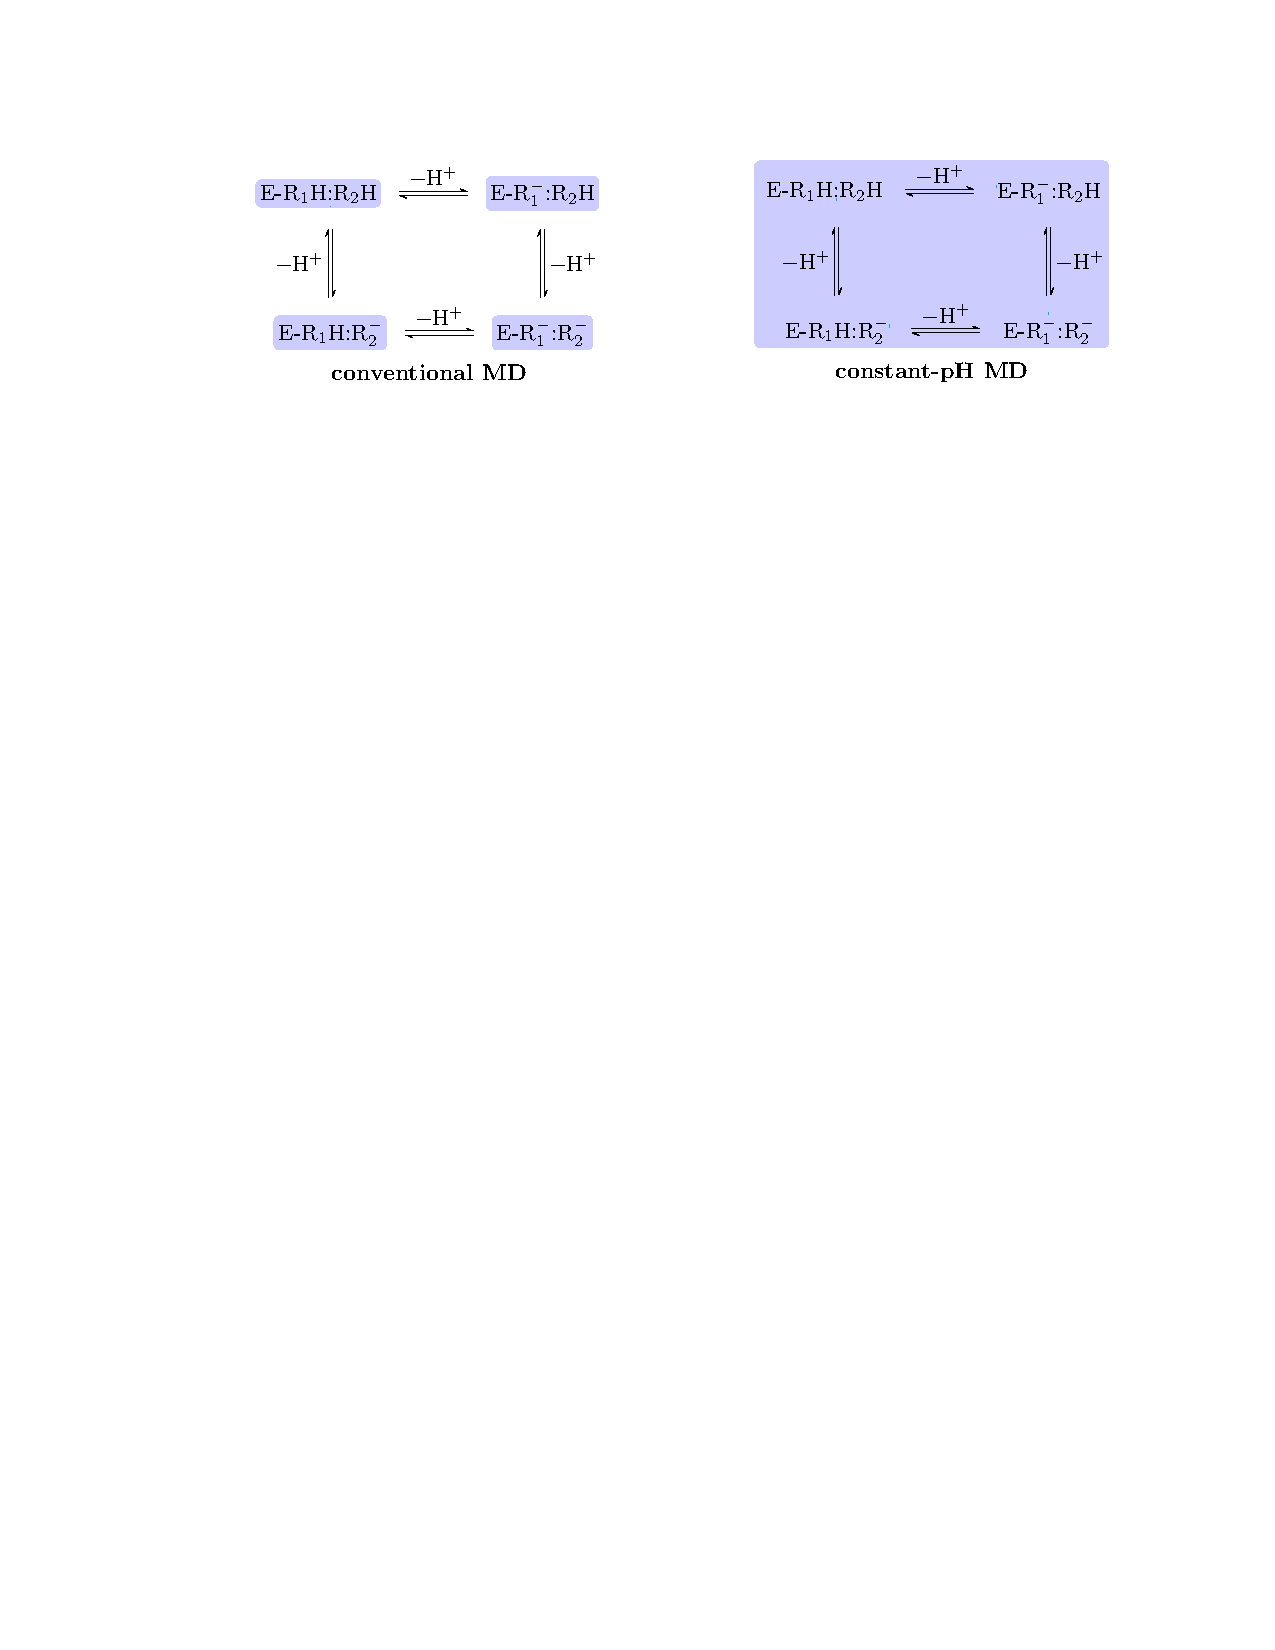
\includegraphics[width=\textwidth]{figures/namdcph_cycle}
  \caption{\label{fig:cphStateCycle}
    The core difference between conventional and constant-pH MD can be
      illustrated by a simple enzyme $E$ with four protonation states
      describing the occupancy of two titratable residues, $R_1$ and $R_2$.
    A conventional MD simulation handles the states \emph{separately} (left
      panel).
    The relative importance of the states must be known beforehand or computed
      by other means.
    Conversely, a constant-pH MD simulation handles the states
      \emph{collectively} and actively simulates interconversion (right panel).
    Determining the relative importance of the states is a direct result of the
      simulation.
  }
}\end{figure}

In formal terms, conventional MD samples from a canonical ensemble, whereas
  constant-pH MD samples from a semi-grand canonical ensemble.
The new partition function,
\begin{equation}\label{eqn:semigrand}
  \Xi(\text{pH})
  =
  \sum_{\text{$\bm \lambda$} \in \mathcal{S}}
    Q_{\text{$\bm \lambda$}}
    10^{-n_{\text{$\bm \lambda$}} \text{pH}},
\end{equation}
  is essentially a weighted summation of canonical partition functions,
  $Q_{\text{$\bm \lambda$}}$, each of which are defined by an occupancy vector,
  ${\bm \lambda}$.
The elements of ${\bm \lambda}$ are either one or zero depending on whether a
  given protonation site is or is not occupied, respectively.
For a vector of length $m$, the set of all protonation states, $\mathcal{S}$,
  has at most $2^m$ members.
In order to sample from the corresponding semi-grand canonical distribution
  function, a simulation must explore \emph{both} the phase space defined by
  the canonical paritition functions and the state space defined by the
  different occupancy vectors.
The fraction of simulation time spent in each state is dictated by the weights
  in the summation and these depend on the pH and the number of protons,
  $n_{\text{$\bm \lambda$}}$, in the system (\textit{i.e.},~the sum of the
  elements in ${\bm \lambda}$).

Although a constant-pH MD system may contain any number of titratable protons,
  the base transformation is always the movement of \emph{one} proton from a
  molecule into a bath of non-interacting protons ``in solution.''
For a generic chemical species A, this corresponds to the usual deprotonation
  reaction definition, except with fixed pH:
\begin{equation*}
 \mathrm{
  HA
  \underset{\text{pH fixed}}{\stackrel{-H^{+}}{\rightleftharpoons}}
  A^{-}
 }.
\end{equation*}
In the language of statistical mechanics the species HA and A$^{-}$ refer to
  all terms in Eq.~\eqref{eqn:semigrand} which do and do not, respectively,
  contain the specific proton in question (\textit{i.e.},~the particular
  element of ${\bm \lambda}$ is one or zero).
By taking out a factor of $10^{-\text{pH}}$, this can be re-written as
\begin{equation*}
  \Xi(\text{pH})
  =
  \Xi_{\text{A}^{-}}(\text{pH})
  +
  \Xi_{\text{HA}}(\text{pH}) 10^{-\text{pH}}
\end{equation*}
  and then recast as a statistical mechanical analog of the 
  Henderson-Hasselbalch equation by recognizing that
  $\Xi_{\text{A}^{-}}(\text{pH}) / \Xi_{\text{HA}}(\text{pH})$ is just the
  ratio of deprotonated / protonated fractions of species A.
The \emph{protonated} fraction is then
\begin{equation}\label{eqn:HH}
  P_{\text{HA}}(\text{pH})
  =
  \frac{1}{1 + 10^{\text{pH} - \pKa(\text{pH})}};
  \qquad
  \pKa(\text{pH})
  \equiv
  -\log{
    \frac{
      \Xi_{\text{A}^{-}}(\text{pH})
    }{
      \Xi_{\text{HA}}(\text{pH})
    }
  }.
\end{equation}
In practice, $P_{\text{HA}}(\text{pH})$ can be calculated from a simulation by
  simply counting the fraction of time spent in state HA (\textit{e.g.},~the
  fraction of time a specific element of ${\bm \lambda}$ is one).
Note also that $\pKa(\text{pH})$ is formally a pH dependent function
  unless the system only contains one proton (or type of proton).

In most experimental contexts, a different form of Eq.~\eqref{eqn:HH} is used
  which is often referred to as a ``generalized'' Hill equation.
This corresponds to a specific choice of pH dependence such that
\begin{equation*}
  \pKa(\text{pH})
  \approx
  \pKaX{(a)}
  +
  (1 - n)\left(\text{pH} - \pKaX{(a)}\right).
\end{equation*}
The constant $n$ is then known as the Hill coefficient and the so-called
  apparent $\pKa$, $\pKaX{(a)}$, generally corresponds to the inflection point
  of a plot of $P_{\text{HA}}(\text{pH})$.
Both quantities are usually determined by non-linear regression after
  $P_{\text{HA}}$ has been determined at different pH values.

\subsection{Implementation Details}

In NAMD, each canonical partition function is represented by a specific force
  field description embodied in a PSF -- in order to change the protonation
  state the underlying PSF must also be modified.
This is accomplished by a close coupling to \texttt{psfgen}.
The models that can be used with constant-pH MD are thus limited to only those
  which can be completely implemented within \texttt{psfgen}.
This also means that NAMD requires access to residue topology files (RTFs)
  during the course of a simulation.
These must be specified with the \texttt{psfgen} \texttt{topology} command.

For consistency between topological descriptions, NAMD uses ``dummy'' atoms to
  represent non-interacting protons.
These atoms have the same mass as protons but only interact with the system
  via a minimal number of force field bonded terms.
This formalism guarantees that:
  1) the number of atoms/coordinates during the simulation remains fixed
  and
  2) the thermodynamics of the model is unchanged.
The latter point is subtle and warrants comment.
As implemented in NAMD, constant-pH MD only captures the thermodynamics of
  the semi-grand canonical ensemble.
There is no active description of proton dissociation events.
However, this is more of a limitation of classical MD than a particular
  shortcoming of NAMD.
A useful analogy may be the use of Langevin dynamics as a thermostat as
  opposed to a phenomonological model for Brownian motion.

\begin{figure}[h]\center{
  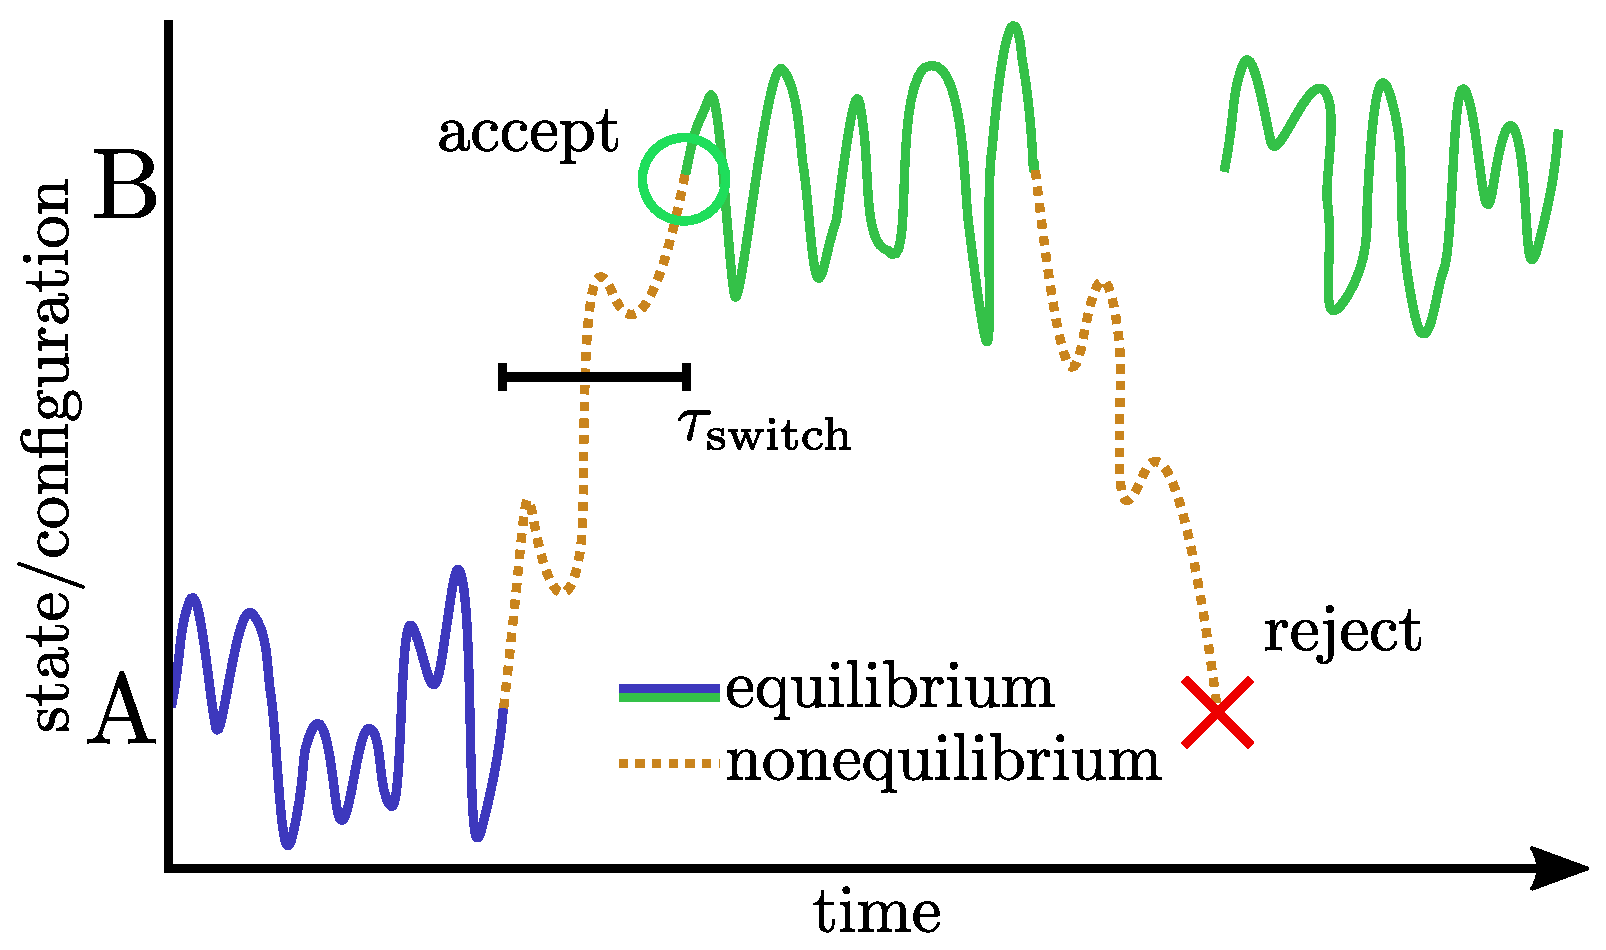
\includegraphics[width=0.6\textwidth]{figures/namdcph_nemdmc_scheme}
  \caption{\label{fig:namdcph_nemdmc}
    The basic constant-pH MD scheme in NAMD is to alternate equilibrium 
      sampling in a fixed protonation state followed by a nonequilibrium MD
      Monte Carlo move to sample other protonation states.      
    The latter move can be accepted or rejected.
    If accepted, the simulation continues in the new protonation state.
    If the move is rejected, sampling continues as if the move were never
      attempted at all.
  }
}\end{figure}

The basic scheme in NAMD is to alternately sample the protonation state and
  then the configuration space within that state.
Protonation state sampling is accomplished by an alchemical coupling scheme
  that forcibly turns off interactions with the current protonation state and
  turns on interactions with a candidate protonation state.
This nonequilibrium ``switching'' is accomplished with the alchemy code 
  (specifically the thermodynamic integration code branch) and necessarily has
  lower performance (by about 30\%) than regular MD due to the added
  electrostatic calculations in the reciprocal space (\textit{i.e.}, when
  using PME).
However, the configuration space sampling should still have normal performance.
The switching process exerts work on the system and thus drives the system out
  of equilibrium.
However, an appropriately designed Monte Carlo (MC) move using an accept/reject
  criterion can recover the correct semi-grand canonical equilibrium 
  distribution in both the state and configuration
  spaces~\cite{Nilmeier_ProcNatlAcadSci_2011_v108_pE1009,
    Chen_JChemPhys_2015_v142_p024101}.
The resulting scheme is a hybrid nonequilibrium MD/MC (neMD/MC) algorithm.
The most important conceptual change from conventional MD is that, rather than
  being a continuous trajectory, the simulation now becomes a series of cycles
  composed of an MD and neMD/MC step.
This means that the length of the simulation is no longer simply determined by
  the number of steps (\texttt{numsteps}) but rather the number of cycles.
The length of a cycle is also determined by two parts -- the amount of time on
  equilibrium sampling and the amount of time executing the switch.

It may be profitable/necessary to vary the switch time depending on the type of
  protonation change that is being effected.
Indeed, this is a critical factor in the efficiency of the method.
That is, if the switch is too short, then moves are unlikely to be accepted and
  effort will be wasted when the move is rejected.
However, if the switch is too long, then an inordinate amount of effort will be
  spent sampling the state space and there will be fewer resources left for
  exploring the configuration space.
Some basic qualities of the system that affect sampling have been determined
  using nonequilibrium linear response
  theory~\cite{Radak_JChemPhys_2016_v145_p134109}.
In short, there are intrinsic limits based on:
  1) the extent that differing interactions between each state fluctuate
  (according to some variance, $\sigma_0^2$)
  and
  2) the ``molecular'' time scale, $\tau_{\text{m}}$, on which these
  fluctuations change.
These effects are roughly captured by the
  expression~\cite{Radak_JChemPhys_2016_v145_p134109,
    Radak_JChemTheoryComput_2017_v13_p5933}:
\begin{equation*}
  \tau_{\text{opt}}
  \le
  \frac{\sigma_0^2 \tau_{\text{m}}}{2.83475},
\end{equation*}
  where $\tau_{\text{opt}}$ is some optimal switching time, in the sense of
  maximizing the rate at which protonation states interconvert.
Overall, switching times on the order of tens of picoseconds tend to be optimal
  in that they balance the high cost of switching versus the high acceptance
  rate at longer switching times (in the infinite time limit the perturbation
  is adiabatic and exerts zero work).
For titratable groups exposed primarily to aqueous solvent, a switch on the
  order of 10-20~ps appears to give near optimal
  results~\cite{Radak_JChemPhys_2016_v145_p134109,
    Radak_JChemTheoryComput_2017_v13_p5933}. 
An equivalent formulation of the above expression is that mean acceptance rates
  around 20-25\% are likely near optimal.

\fbox{
  \begin{minipage}[ht!]{15.3cm}
    \addtolength{\baselineskip}{0.225\baselineskip}
    \textbf{Important Limitations:}\\
    For various reasons concerning the implementation, constant-pH simulations
      are currently \emph{incompatible} with the following NAMD
      functionalities in all or most situations:
    \begin{itemize}
    \item Any system using GPUs/CUDA
    \item Generalized Born implict solvent (\texttt{GBIS})
    \item Alchemical free energy calculations, \textit{e.g.},~ligand binding
      (\texttt{alch})
    \item Drude polarizable force fields
    \item Hybrid quantum mechanical/molecular mechanical simulations
    \item Collective variables (\texttt{colvars})
    \item \texttt{extraBonds}
    \end{itemize}
    This list is neither exhaustive nor definitive.
    In many instances the problem may be overcome by modest additional
      developments. %(see Notes for Developers).
  \end{minipage}
}

\newpage
\begin{center}
  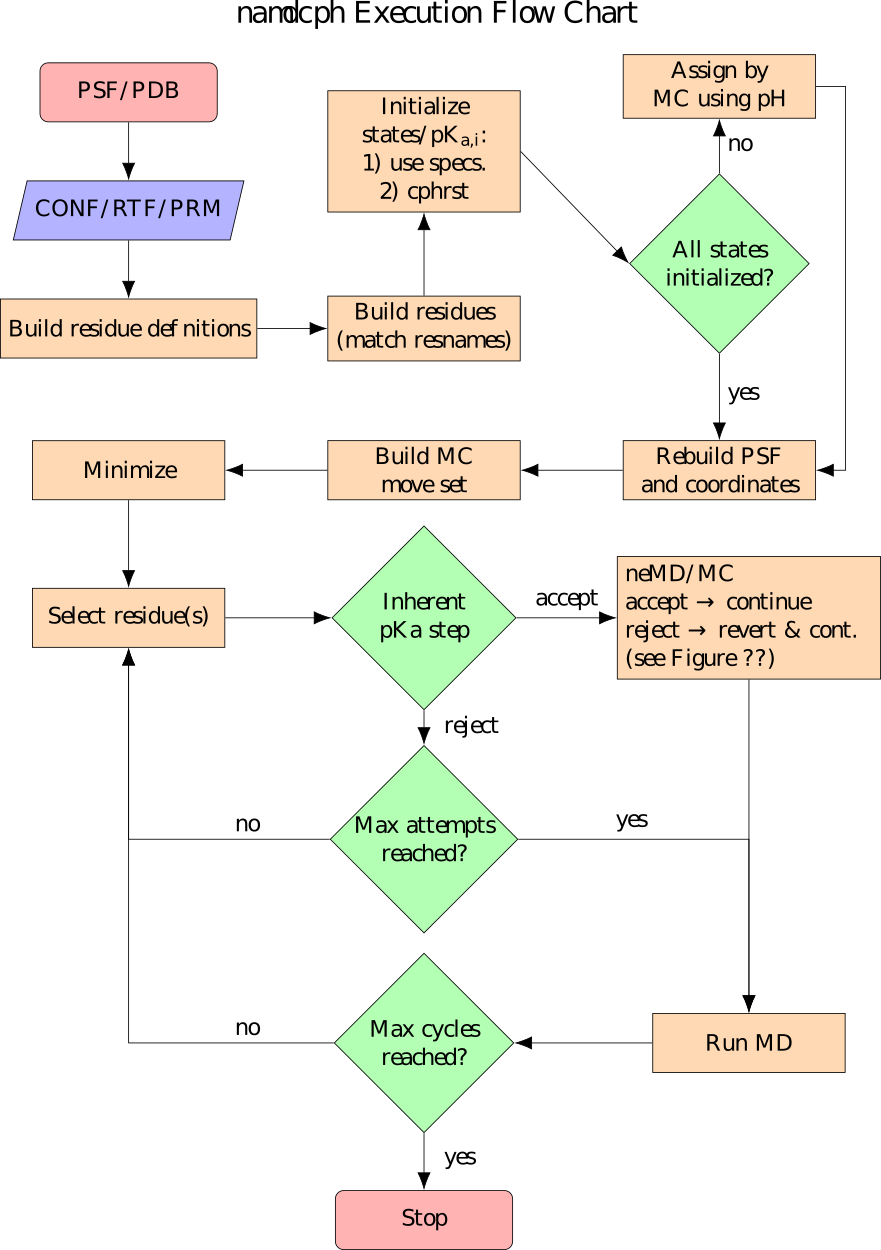
\includegraphics[width=0.9\textwidth]{figures/namdcph_flowchart}
\end{center}

\newpage
\subsection{New Commands and Keywords}

The constant-pH implementation is largely implemented in Tcl and can be found
  in \texttt{/lib/namdcph/namdcph.tcl}, where the base directory is the NAMD
  source home directory.
When that file has been loaded with a suitable \texttt{source} command, the 
  following commands and keywords are available and appear to the user in a way
  similar to NAMD syntax.
The most significant change from normal NAMD usage is that there is generally
  no need to use the \texttt{run} command.
One should instead use the new \icommand{{\tt cphRun}} command;
this can only be used \emph{once} per script for now.
\textit{NB}, all commands and keywords are currently case sensitive!
\\[11pt]
\noindent
\icommand{{\tt cphRun}} $<$ Run constant-pH MD $>$
\\
\textbf{Arguments:} {\ARG{numsteps} \OARG{numcycles}}
\\
\textbf{Defaults:} {{\tt numcycles} = 1}
\\
\textbf{Description:}
Execute {\tt numcycles} cycles of constant-pH MD with the current settings.
Each cycle consists of 1) a neMD/MC move in both configuration and protonation
  space and 2) MD based sampling in configuration space.
By default, configuration space sampling simply consists of {\tt numsteps}
  dynamics, as in conventional MD.
The nature of the neMD/MC moves, however, is more elaborate and controlled by
  other keywords, \emph{many of which are required} (see below).
%\\[11pt]
%\noindent
%\icommand{{\tt testResidue}} $<$ Test a constant-pH residue definition $>$
%\\
%\textbf{Arguments:} {\ARG{resname list} \OARG{verbose}}
%\\
%\textbf{Defaults:} {{\tt verbose} = 0}
%\\
%\textbf{Description:}
%THIS IS AN ADVANCED OPTION, USE WITH CARE!
%This is meant to be a convenience command for verifying that RTF, PRM, and
%  configuration file definitions are complete and consistent.
%The \texttt{resname list} argument should be a Tcl list containing the names
%  of one or more residue definitions described in the configuration file.
%Accompanying \texttt{parameter} and \texttt{topology} information is also
%  required, as in normal simulations.
%The command will iterate through all possible protonation state transitions and
%  check that the energy of each state does not depend on the pathway by which
%  it is reached.
%Setting {\tt verbose} $\ne$ 0 will also show decomposition of energy terms
%  (\textit{e.g.}, ELEC and VDW).

\subsubsection{Required Keywords}
\begin{itemize}
\item \NAMDCONF{pH}
{pH value that the system is in contact with}
{decimal (usually between 0 and 14)}
{
The \KEY{pH} is effectively a chemical potential applied to protons
  \emph{only}.
This value affects the details of neMD/MC moves but otherwise has no effect
  on the system dynamics.
}

\item \NAMDCONF{cphConfigFile}
{File defining titratable residues}
{filename}
{
The \KEY{cphConfigFile} contains definitions for the available titratable 
  residues.
This is essentially meta information regarding the RTF contents, but also
  includes experimental references and additional force field parameterization.
}

\item \NAMDCONF{cphNumstepsPerSwitch}
{Number of steps during nonequilibrium switching}
{
  \OARG{integer \OARG{\ARG{move label} \ARG{integer}} \ldots}
}
{
Each move must have an associated number of steps per switch. 
If an odd number number of arguments is specified, then the first such argument
  is assumed to be a default number for all such moves.
After this (or if an even number of arguments is specified) all remaining
  arguments are assumed to be specific assignments for a given move label
  of the form \ARG{segid}:\ARG{resid}:\ARG{resname}/\ARG{segid}:\ARG{resid}:\ARG{resname}/\ldots.
}
\end{itemize}

\subsubsection{Commonly Used Options}
\begin{itemize}
\item \NAMDCONF{cphSetResidueState}
{Set the initial state of one or more titratable residues.}
{
\ARG{segid}:\ARG{resid}:\ARG{resname} \ARG{state} \OARG{\ldots}
}
{
Initial residue states can be assigned in three ways (in descending order of 
  precedence): 1) via this command, 2) from a \KEY{cphRestartFile}, and 3)
  randomly from the assigned \KEY{pH} and the current inherent pKa of each
  residue.
}

\item \NAMDCONF{cphSetResiduepKai}
{Set the inherent pKa of one or more titratable residues.}
{
\ARG{segid}:\ARG{resid}:\ARG{resname} \ARG{pKai} \OARG{\ldots} 
}
{
The two step inherent pKa algorithm implemented here permits on-the-fly update
  of an estimate for the pKa(s) of each residue.
These can either be guessed at the outset (the default is to use the reference
  pKa) or updated as the simulation progresses.
A more accurate estimate of the inherent pKa increases the statistical
  efficiency of the method, but the long time result is formally unbiased
  regardless of the value.
If an extremely large or extremely small value is assigned, then the residue
  will be assigned the most probable protonation state at the given pH and
  likely remain fixed in that state.
}

\item \NAMDCONF{cphExcludeResidue}
{Exclude one or more residues from being titratable}
{
\ARG{segid}:\ARG{resid}:\ARG{resname} \OARG{\ldots}
}
{
By default, any residue that matches a titratable residue type will be allowed
  to change protonation state.
This command permits specific residues to be excluded from consideration in a
  manner that is similar to assigning an extreme inherent pKa (see
  \texttt{cphSetResiduepKai}).
The main differences are that 1) the protonation state will not be modified and
  remain as it is in the original PSF and 2) the protons in the residue will
  \emph{not} be tracked in the \texttt{cphlog} file.
This command is not always recommended, but is currently necessary for handling
  disulfide linkages.
}

\item \NAMDCONF{cphRestartFile}
{Restart file for constant-pH}
{filename}
{
Constant pH requires additional checkpoint information regarding the state of
  the titratable residues and the nature of the neMD/MC moves.
This (optional) information is read from the file specified here.
After/during a simulation, this information is written to 
  \KEY{[outputname]}.cphrst.
}

\item \NAMDCONFWDEF{cphRestartFreq}
{Frequency at which constant-pH checkpoint files are written}
{Non-negative integer}
{0}
{
Checkpoint information is written to \KEY{[outputname]}.cphrst every 
  \KEY{cphRestartFreq} cycles (\emph{not} MD steps).
A checkpoint file is \emph{always} written at the end of the last cycle.
}

\item \NAMDCONFWDEF{cphOutFile}
{Log file for constant-pH}
{filename}
{\KEY{[outputname]}.cphlog}
{Titratable residue state information is logged here after every cycle.}

\item \NAMDCONF{cphProposalWeight}
{MC move label and weight specifications}
{
\ARG{move label} \ARG{weight}
  \OARG{\OARG{\ARG{move label} \ARG{weight}} \ldots}
}
{
During each cycle, MC moves are selected from the move set and then 
  accepted/rejected according to a Metropolis criterion based on the combined 
  inherent pKa information and pH.
The move weight affects the probability that such a move is selected. 
Note that \emph{this does not affect the probability that any given proposal
  is accepted}, it merely increases the number of attempts at the given
  proposal.
This may be useful in a system where one desires specific attention on a given
  process, such as proton transfer or the exchange of a given residue, but one
  does not want to assume that all other residue protonation states are
  nominally fixed.
By default all moves are assigned equal weights of 1.0.
During the simulation these are automatically normalized to a discrete
  probability mass function.
}

\item \NAMDCONFWDEF{cphMaxProposalAttempts}
{Maximum number of switch proposal attempts per cycle}
{integer}
{0}
{
During each cycle, MC moves are selected from the move set and then
  accepted/rejected according to a Metropolis criterion based on the combined
  inherent pKa information and pH.
This process stops when either a switch move is accepted or a maximum limit is
  reached.
Any value less than one defaults to the number of titratable residues in the
  system.
}

\item \NAMDCONFWDEF{cphNumMinSteps}
{Number of steps of minimization before dynamics}
{integer}
{0}
{
This is a replacement for the normal minimize command, which is not compatible
  with constant-pH due to PSF modifications during initialization.
Setting this option to a modest number (100--200, say) might be necessary when
  randomizing protonation states based on pH, since in that case it cannot be
  assumed that the starting structure is representative of the initial
  protonation state.
}

\end{itemize}

\subsubsection{Specialized Options}
\begin{itemize}
\item \NAMDCONFWDEF{cphForceConstant}
{force constant for alchemical switches (in kcal/mol-\AA$^2$)}
{Non-negative decimal}
{100.0}
{
During ``dual-topology'' alchemical switches, a harmonic bond is formed between
  analogous atoms in each alchemical region.
This rigorously leaves all static thermodynamic quantities intact and is
  generally expected to improve the stability of dynamic quantities.
}

\item \NAMDCONFWDEF{cphMDBasename}
{basename of intermediate files for equilibrium MD}
{string}
{namdcph.md}
{
PSF/coordinate modifications are currently done via the file system and utilize 
  intermediate files.
It may be advantageous to direct this I/O to a fast temporary directory.
}

\item \NAMDCONFWDEF{cphSWBasename}
{basename of intermediate files for nonequilibrium (switch) MD}
{string}
{namdcph.sw}
{
PSF/coordinate modifications are currently done via the file system and utilize
  intermediate files.
It may be advantageous to direct this I/O to a fast temporary directory.
}
\end{itemize}

\fbox{
  \begin{minipage}[ht!]{15.3cm}
    \addtolength{\baselineskip}{0.225\baselineskip}
    \textbf{Undocumented Features:}\\
    The constant-pH code is actively under development, although future work
      will almost exclusively be in adding new features and capabilities as
      well as improving performance.
    Because the code is fairly lightweight and available in \texttt{Tcl}, the
      intrepid user may discover ``easter egg'' features which are not listed
      in the documentation.
    \textbf{USE UNDOCUMENTED FEATURES AT YOUR OWN RISK.}
    Such undocumented features may work (and even be advisable) for specific
      problems, but have not undergone as rigorous of testing and may be prone
      to unintended consequences.
  \end{minipage}
}

\subsection{Minimal Examples}

Constant-pH simulations can be carried out with largely the same options as
  conventional MD simulations (with some exceptions, see previous sections).
The follwing examples assume that: 1) PSF and PDB files for the
  system of interest have already been constructed and 2) appropriate
  simulation keywords have already been chosen (\textit{e.g.},~for PME,
  Langevin dynamics, \textit{etc.}).
\begin{verbatim}
# End conventional settings...
source .../namd/lib/namdcph/namdcph.tcl
# Constant-pH MD requires additional force field files _during_ the simulation.
# In general, all RTFs used to construct the system need to be included with
# the ``topology'' command (just as in psfgen). Additional constant-pH specific
# RTF and PRM files are also necessary, as well as an accompanying
# configuration file in JSON format.
#
cphConfigFile <path to JSON config file>
topology <path to RTF>
topology <path to another RTF>
pH 7.0
# The following defaults all nonequilibrium switches to 5000 steps and then
# increases the time for residue 5 of segid PROA to 7500 steps -- multiple
# residues can be specified 
#
cphNumStepsPerSwitch 5000 PROA:5:ASP 7500
# Run 100 minimization cycles before starting dynamics.
cphNumMinSteps 100
# Run 2500 steps of MD between attempted protonation state changes. Run 10
# cycles of MD and neMD/MC. The _upper_ bound of the simulation is thus:
#
# 10*(2500 + 7500) = 100000 steps
#
# but the actual simulation may be shorter in length.
#
cphRun 2500 10
\end{verbatim}

\newpage
\noindent
\textbf{Restarting a simulation}

\noindent
The following assumes that a simulation has already been run (as in the example
  above).
For clarity we shall assume that \texttt{outputname} was set to "foo" such that
  restart files have been written to foo.coor and foo.vel (normal output) as
  well as foo.psf, foo.pdb, and foo.cphrst (constant-pH specific output).

\begin{verbatim}
# End conventional settings...
source .../namd/lib/namdcph/namdcph.tcl
# Constant-pH MD requires additional force field files _during_ the simulation.
# In general, all RTFs used to construct the system need to be included with
# the ``topology'' command (just as in psfgen). Additional constant-pH specific
# RTF and PRM files are also necessary, as well as an accompanying
# configuration file in JSON format.
#
cphConfigFile <path to JSON config file>
topology <path to RTF>
topology <path to another RTF>
pH 7.0

structure foo.psf
coordinates foo.pdb
binCoordinates foo.coor
binVelocities foo.vel
cphRestartFile foo.cphrst
# NB: switch times and inherent pKa values are read here and no longer need to
# be specified as during initialization

cphRun 2500 10
\end{verbatim}

%% COMING SOON
%\newpage
%\subsection{Notes for Developers}
%
%This section of the user's guide is likely not necessary reading for those
%  who simply want to perform constant-pH simulations.
%Rather, it is a companion guide for the code and comments so that furthur
%  developments can be made as a community.

